\section{Results}
\label{sec:results}

Completed multi-seed results cover LastFM Asia, Facebook Page-Page, and GitHub Developers ($n{=}10$ seeds; budgets $0.1$--$0.9$; $1{,}890$ authoritative rows).

\subsection{Main multi-seed sparsification results}
Figure~\ref{fig:curves} and Table~\ref{tab:main} report Macro-F1 versus edge-removal rate ($n{=}10$ seeds on all three datasets).

\begin{figure}[t]
\centering
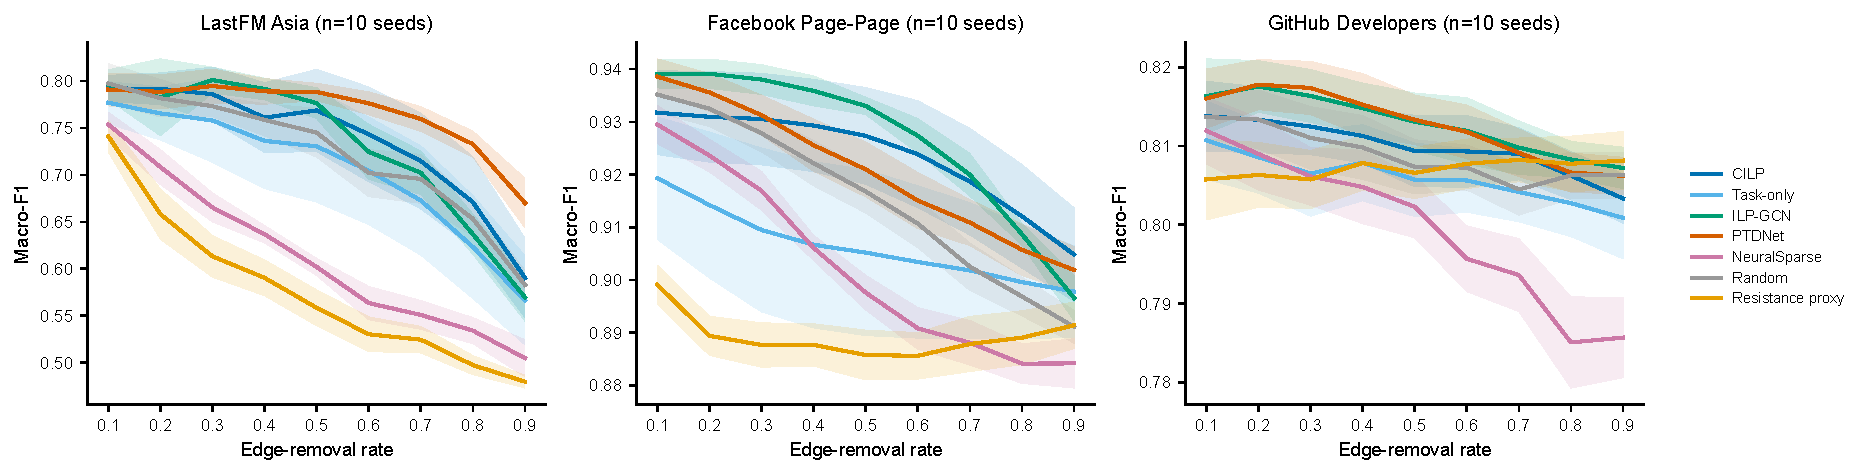
\includegraphics[width=\linewidth]{figures/fig2_sparsity_curves.pdf}
\caption{\textbf{Sparsity--Macro-F1 curves.}
Mean Macro-F1 versus edge-removal rate; bands are $95\%$ $t$-intervals (mean $\pm t_{0.975,n-1}\mathrm{SEM}$) with $n{=}10$ seeds.
Panels use dataset-specific $y$-axis ranges.
Curves begin at $10\%$ removal; a full-graph ($0\%$) reference is not included in the present grid.
Legend order: CILP, Task-only, ILP-GCN, PTDNet, NeuralSparse, Random, Resistance proxy.}
\label{fig:curves}
\end{figure}

\begin{table}[t]
\centering
\caption{\textbf{Main predictive results} (mean$\pm$s.d., $n{=}10$ seeds $0$--$9$).
AUC: trapezoidal sparsity--Macro-F1 area over edge-removal rates $0.1$--$0.9$.
\textbf{Bold}: best mean in each column within a dataset; \underline{underline}: second-best (ties shared).
Visual ranking does not imply statistical significance.}
\label{tab:main}
\scriptsize
\begin{tabular}{@{}llcccc@{}}
\toprule
Dataset & Method & 30\% & 50\% & 70\% & AUC \\
\midrule
\multirow{7}{*}{LastFM}
& PTDNet & $\underline{0.795}{\pm}0.025$ & $\textbf{0.788}{\pm}0.013$ & $\textbf{0.760}{\pm}0.018$ & $\textbf{0.616}{\pm}0.011$ \\
& CILP & $0.786{\pm}0.040$ & $0.769{\pm}0.061$ & $\underline{0.715}{\pm}0.071$ & $\underline{0.593}{\pm}0.038$ \\
& ILP-GCN & $\textbf{0.801}{\pm}0.019$ & $\underline{0.776}{\pm}0.023$ & $0.702{\pm}0.032$ & $0.590{\pm}0.017$ \\
& Random & $0.773{\pm}0.016$ & $0.745{\pm}0.036$ & $0.696{\pm}0.036$ & $0.580{\pm}0.018$ \\
& Task-only & $0.758{\pm}0.062$ & $0.730{\pm}0.083$ & $0.673{\pm}0.081$ & $0.566{\pm}0.050$ \\
& NeuralSparse & $0.665{\pm}0.022$ & $0.602{\pm}0.013$ & $0.551{\pm}0.021$ & $0.489{\pm}0.010$ \\
& Resistance proxy & $0.613{\pm}0.031$ & $0.558{\pm}0.027$ & $0.524{\pm}0.020$ & $0.458{\pm}0.014$ \\
\midrule
\multirow{7}{*}{Facebook}
& ILP-GCN & $\textbf{0.938}{\pm}0.004$ & $\textbf{0.933}{\pm}0.002$ & $\textbf{0.920}{\pm}0.006$ & $\textbf{0.742}{\pm}0.003$ \\
& CILP & $\underline{0.931}{\pm}0.012$ & $\underline{0.927}{\pm}0.013$ & $\underline{0.919}{\pm}0.014$ & $\underline{0.739}{\pm}0.010$ \\
& PTDNet & $\underline{0.931}{\pm}0.005$ & $0.921{\pm}0.007$ & $0.911{\pm}0.006$ & $0.737{\pm}0.004$ \\
& Random & $0.928{\pm}0.005$ & $0.917{\pm}0.006$ & $0.903{\pm}0.006$ & $0.732{\pm}0.004$ \\
& Task-only & $0.909{\pm}0.022$ & $0.905{\pm}0.022$ & $0.902{\pm}0.018$ & $0.725{\pm}0.015$ \\
& NeuralSparse & $0.917{\pm}0.005$ & $0.898{\pm}0.005$ & $0.888{\pm}0.006$ & $0.721{\pm}0.003$ \\
& Resistance proxy & $0.888{\pm}0.006$ & $0.886{\pm}0.007$ & $0.888{\pm}0.007$ & $0.711{\pm}0.005$ \\
\midrule
\multirow{7}{*}{GitHub}
& ILP-GCN & $\underline{0.816}{\pm}0.005$ & $\textbf{0.813}{\pm}0.005$ & $\textbf{0.810}{\pm}0.005$ & $\textbf{0.650}{\pm}0.003$ \\
& PTDNet & $\textbf{0.817}{\pm}0.005$ & $\textbf{0.813}{\pm}0.004$ & $\underline{0.809}{\pm}0.004$ & $\textbf{0.650}{\pm}0.003$ \\
& CILP & $0.812{\pm}0.005$ & $\underline{0.809}{\pm}0.006$ & $\underline{0.809}{\pm}0.005$ & $\underline{0.648}{\pm}0.004$ \\
& Random & $0.811{\pm}0.006$ & $0.807{\pm}0.005$ & $0.804{\pm}0.005$ & $0.647{\pm}0.003$ \\
& Resistance proxy & $0.806{\pm}0.005$ & $0.807{\pm}0.005$ & $0.808{\pm}0.004$ & $0.646{\pm}0.004$ \\
& Task-only & $0.807{\pm}0.008$ & $0.806{\pm}0.007$ & $0.804{\pm}0.005$ & $0.645{\pm}0.004$ \\
& NeuralSparse & $0.806{\pm}0.005$ & $0.802{\pm}0.005$ & $0.794{\pm}0.006$ & $0.640{\pm}0.005$ \\
\bottomrule
\end{tabular}
\end{table}

\subsection{Comparison with ILP-GCN and learned sparsifiers}
Figure~\ref{fig:compare} shows paired CILP AUC differences against Task-only, ILP-GCN, and PTDNet.
On LastFM, PTDNet leads mean AUC; CILP is competitive with ILP-GCN.
On Facebook, ILP-GCN leads slightly, with CILP and PTDNet close behind.
On GitHub, CILP significantly improves over Task-only but remains slightly below ILP-GCN and PTDNet in predictive AUC
(paired $\Delta\approx-0.0024$ and $-0.0023$; Supplementary Information~S16--S18).

\begin{figure}[t]
\centering
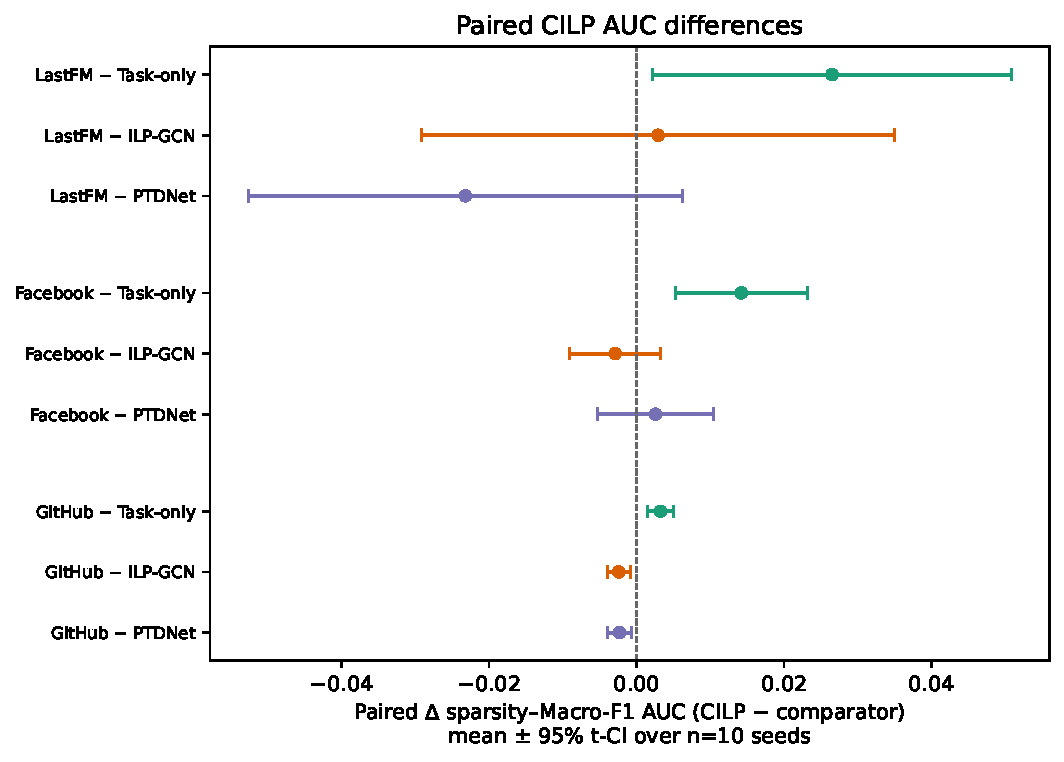
\includegraphics[width=\linewidth]{figures/fig3_method_comparison.pdf}
\caption{\textbf{Paired CILP AUC differences.}
Forest plot of mean CILP$-$comparator sparsity--Macro-F1 AUC with $95\%$ $t$-based CIs ($n{=}10$ seeds).
Positive values favour CILP.}
\label{fig:compare}
\end{figure}

\subsection{Multi-criteria versus task-only counterfactual supervision}
We tested whether combining multiple deletion-importance criteria improves edge ranking relative to task-only supervision under the same encoder, fusion architecture, optimization procedure, removal budgets, and paired seeds.
We considered multi-criteria supervision supported across datasets when it improved at least two seed-aligned evaluation dimensions on at least two datasets under an identical fusion architecture, with Holm adjustment within each dataset's four-metric family~(i) (sparsity--Macro-F1 AUC; giant-component ratio, bridge retention, and minority-degree retention at $50\%$ removal).

On paired seeds $0$--$9$ ($n{=}10$) with concatenation fusion, CILP improves all four metrics over Task-only on LastFM, Facebook, and GitHub (Holm-adjusted Wilcoxon $p{<}0.05$ in family~(i); Supplementary Information~S21; Fig.~\ref{fig:teacher}, Table~\ref{tab:teacher}).
On GitHub the predictive AUC effect is statistically consistent but small in magnitude ($\Delta{=}{+}0.0033$; wins/ties/losses $10/0/0$); statistical significance should not be equated with practical dominance.
The fixed four-metric support criterion is met on all three datasets.
This support is relative to the matched Task-only teacher and does not imply that CILP outperforms all established sparsifiers.

\begin{figure}[t]
\centering
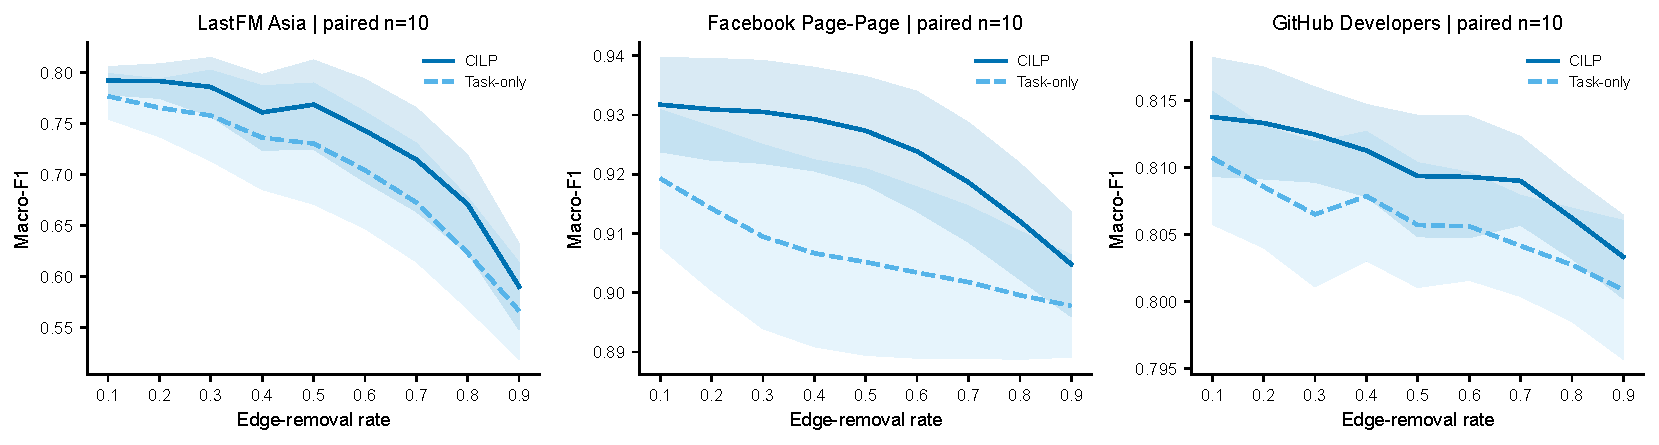
\includegraphics[width=\linewidth]{figures/fig4_teacher_compare.pdf}
\caption{\textbf{Multi-criteria versus task-only supervision.}
Comparison on paired seeds using identical GCN encoders and concatenation fusion ($n{=}10$).
Bands: $t$-based $95\%$ CIs.}
\label{fig:teacher}
\end{figure}

\begin{table}[t]
\centering
\caption{\textbf{Multi-criteria versus task-only counterfactual supervision}
(sparsity--Macro-F1 AUC; paired seeds $0$--$9$).}
\label{tab:teacher}
\scriptsize
\begin{tabular}{@{}lccccccc@{}}
\toprule
Dataset & CILP AUC & Task-only AUC & Paired $\Delta$ & 95\% CI & Wilcoxon $p$ & Holm $p$ & $d_z$ \\
\midrule
LastFM & $0.593{\pm}0.038$ & $0.566{\pm}0.050$ & $+0.0265$ & $[0.0022,0.0508]$ & $0.003906$ & $0.007812$ & $0.781$ \\
Facebook & $0.739{\pm}0.010$ & $0.725{\pm}0.015$ & $+0.0142$ & $[0.0053,0.0231]$ & $0.003906$ & $0.015625$ & $1.137$ \\
GitHub & $0.648{\pm}0.004$ & $0.645{\pm}0.004$ & $+0.0033$ & $[0.0015,0.0051]$ & $0.001953$ & $0.007812$ & $1.292$ \\
\bottomrule
\end{tabular}
\end{table}

\noindent
Win/tie/loss counts for AUC are $9/0/1$ (LastFM), $9/0/1$ (Facebook), and $10/0/0$ (GitHub).

\subsection{Structural and group-preservation results}
At $50\%$ edge removal, CILP preserves connectivity and bridges substantially better than the task-only teacher on all three datasets (Fig.~\ref{fig:structure}, Table~\ref{tab:structure}).
Table~\ref{tab:structure_multi} extends giant-component and bridge retention to $30\%$, $50\%$, and $70\%$ removal so that structural reporting is not restricted to a single operating point.
On GitHub, CILP$-$Task-only differences at $50\%$ are $\Delta_{\mathrm{GC}}{=}{+}0.228$, $\Delta_{\mathrm{bridge}}{=}{+}0.320$, and $\Delta_{\mathrm{mindeg}}{=}{+}0.114$ (Holm $p{=}0.0078$ each in family~(i); W/T/L $=10/0/0$, $10/0/0$, and $9/0/1$).
These structural improvements relative to Task-only are larger than the GitHub predictive AUC gain.
However, CILP is not the overall structural leader: on GitHub, ILP-GCN and PTDNet exceed CILP on giant-component ratio, PTDNet leads minority-degree retention, and CILP leads bridge retention among the reported methods.
On LastFM and Facebook, ILP-GCN likewise remains strong on several structural metrics.
These results support the value of multi-criteria supervision relative to its matched ablation, but not overall structural dominance.
No direct community-preservation metric is currently reported; community enters only as a community-boundary teacher proxy (Supplementary Information~S6).

\begin{figure}[t]
\centering
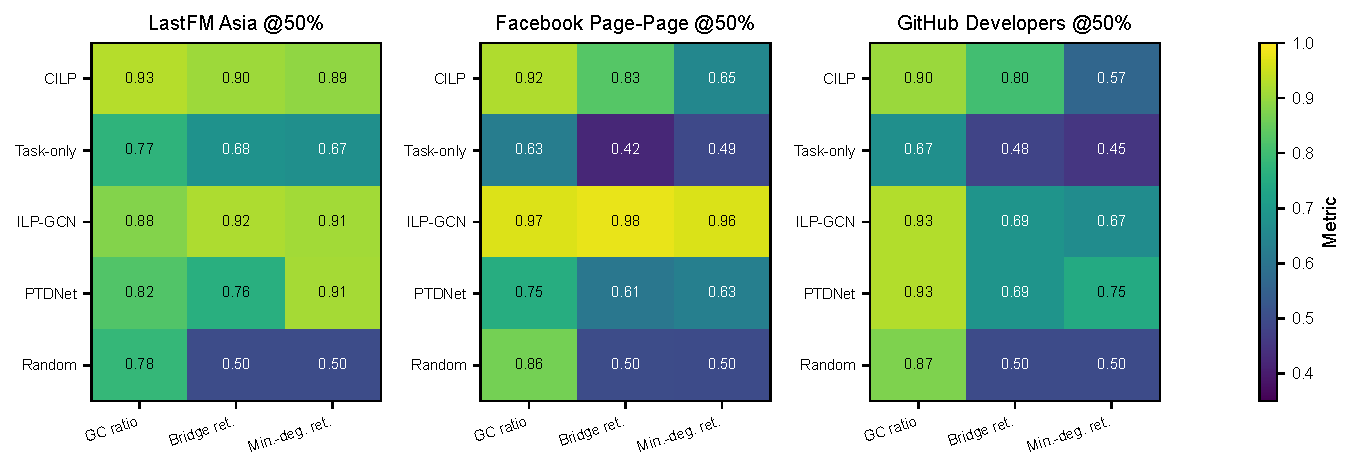
\includegraphics[width=\linewidth]{figures/fig5_structure.pdf}
\caption{\textbf{Structural and group metrics at $50\%$ edge removal} (seed-wise means, $n{=}10$).
Rows denote methods and columns denote metrics.
Cell colours encode metric values using the shared numerical colour scale shown on the right ($[0.35,1.0]$).}
\label{fig:structure}
\end{figure}

\begin{table}[t]
\centering
\caption{\textbf{Structural and group metrics at $50\%$ removal} (means over common seeds).}
\label{tab:structure}
\input{tables/table4_structure.tex}
\end{table}

\begin{table}[t]
\centering
\caption{\textbf{Structural metrics at $30\%$, $50\%$, and $70\%$ removal} (means over $n{=}10$ seeds).
GC: giant-component ratio; Br: bridge retention.}
\label{tab:structure_multi}
\scriptsize
\begin{tabular}{@{}llcccccc@{}}
\toprule
Dataset & Method & GC@30 & GC@50 & GC@70 & Br@30 & Br@50 & Br@70 \\
\midrule
LastFM & CILP & 0.966 & 0.928 & 0.714 & 0.933 & 0.904 & 0.811 \\
LastFM & Task-only & 0.872 & 0.772 & 0.575 & 0.763 & 0.681 & 0.574 \\
LastFM & ILP-GCN & 0.982 & 0.880 & 0.622 & 0.985 & 0.920 & 0.720 \\
LastFM & PTDNet & 0.949 & 0.822 & 0.554 & 0.889 & 0.759 & 0.566 \\
LastFM & Random & 0.894 & 0.784 & 0.602 & 0.700 & 0.501 & 0.300 \\
\midrule
Facebook & CILP & 0.947 & 0.923 & 0.844 & 0.848 & 0.827 & 0.793 \\
Facebook & Task-only & 0.721 & 0.626 & 0.534 & 0.450 & 0.422 & 0.397 \\
Facebook & ILP-GCN & 0.997 & 0.966 & 0.695 & 0.993 & 0.979 & 0.883 \\
Facebook & PTDNet & 0.903 & 0.754 & 0.550 & 0.793 & 0.607 & 0.422 \\
Facebook & Random & 0.937 & 0.863 & 0.731 & 0.703 & 0.502 & 0.300 \\
\midrule
GitHub & CILP & 0.930 & 0.903 & 0.865 & 0.811 & 0.802 & 0.795 \\
GitHub & Task-only & 0.784 & 0.674 & 0.576 & 0.523 & 0.483 & 0.461 \\
GitHub & ILP-GCN & 0.950 & 0.925 & 0.878 & 0.753 & 0.685 & 0.597 \\
GitHub & PTDNet & 0.951 & 0.925 & 0.870 & 0.757 & 0.687 & 0.589 \\
GitHub & Random & 0.941 & 0.873 & 0.750 & 0.700 & 0.500 & 0.299 \\
\bottomrule
\end{tabular}

\end{table}

\subsection{Surrogate quality and uncertainty estimation}
Surrogate--teacher agreement is higher under the multi-criteria teacher than under Task-only on LastFM and Facebook.
On GitHub, CILP attains higher Spearman and Kendall rank agreement, while Task-only has lower raw MAE and ECE is essentially equal (Supplementary Information~S19).
Because pruning ranks edges, rank agreement is the more relevant surrogate diagnostic than absolute regression error; lower MAE alone does not imply a better deletion ranking.
Ranking uses $\mu_e$; $\sigma_e$ is estimated uncertainty and is not an uncertainty-aware pruning rule in reported runs (Supplementary Information~S10).

\subsection{Ablation studies}
LastFM ablations (seeds $0$--$4$; $n{=}5$) are summarized in Fig.~\ref{fig:ablate} by fusion, priors, teacher, and a contextual parent-method comparison.
The Fusion panel holds the multi-criteria teacher fixed and compares concatenation, gated fusion, and cross-attention.
The Teacher panel compares multi-criteria versus task-only under concatenation.
The Context panel contrasts CILP with ILP-GCN and is not a matched ablation.
Leave-one-criterion-out and weight-sensitivity analyses are recommended next steps and are not claimed in the present results.
Adversarial variants were omitted after a negative pilot (Supplementary Information~S20).

\begin{figure}[t]
\centering
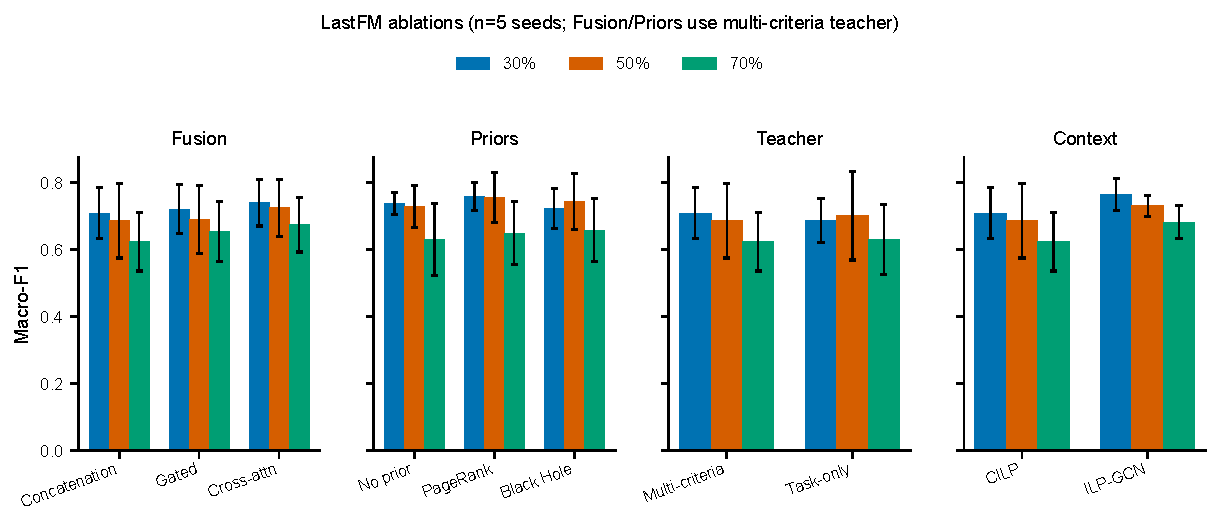
\includegraphics[width=\linewidth]{figures/fig6_ablations.pdf}
\caption{\textbf{LastFM ablations} ($n{=}5$ seeds $0$--$4$).
Fusion and Teacher panels use the multi-criteria teacher unless noted; Context compares CILP with ILP-GCN.
The Priors panel shows a selected subset of three completed prior variants (no prior, PageRank, Black Hole); the full five completed prior variants appear in Supplementary Information~S20.}
\label{fig:ablate}
\end{figure}

\subsection{Runtime}
Wall-clock training times for CILP and Task-only include teacher construction and scorer fitting and were not logged separately (Fig.~\ref{fig:runtime}, Table~\ref{tab:runtime}).
CILP training is therefore substantially more expensive than ILP-GCN and PTDNet on all three datasets, but we do not claim that teacher construction alone dominates that cost.
The full GitHub grid orchestration wall-clock was approximately $6.19$\,h; that figure is an orchestration-level total, not a single method's mean runtime.
Successful completion on GitHub ($37{,}700$ nodes; $289{,}003$ unique undirected edges) demonstrates feasibility at this scale under the reported CPU protocol; it does not establish large-scale GPU efficiency or quantify downstream training speedup after sparsification.

\begin{figure}[t]
\centering
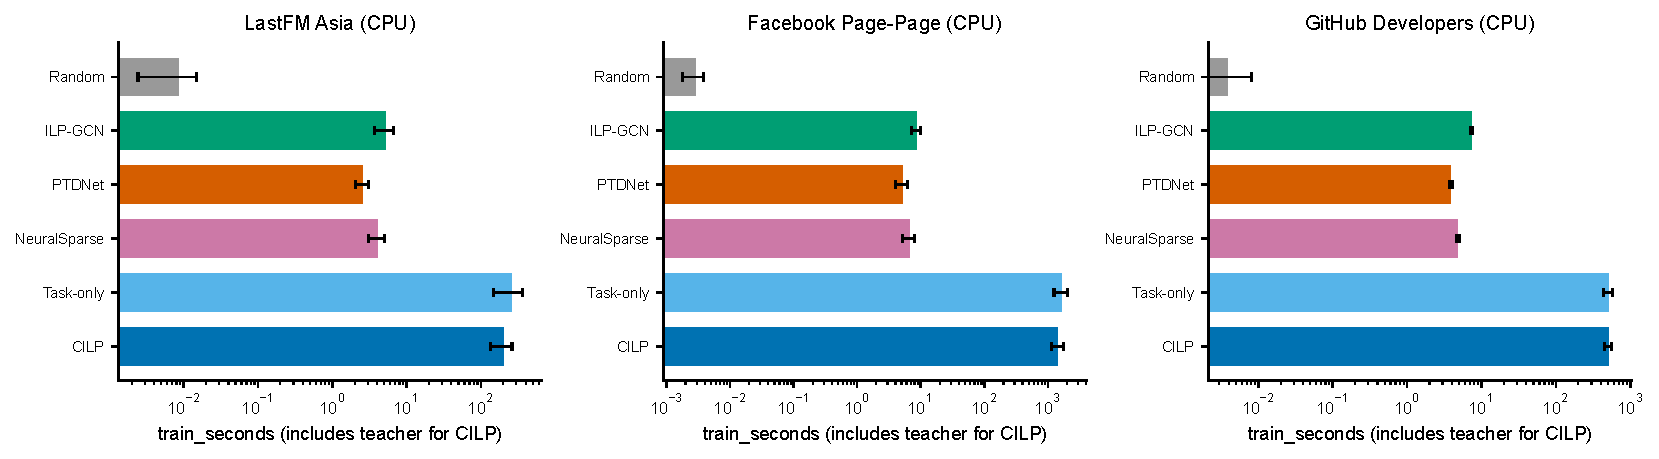
\includegraphics[width=\linewidth]{figures/fig7_runtime.pdf}
\caption{\textbf{Training wall-clock} (CPU, log scale; $n{=}10$).
CILP/Task-only times include the counterfactual teacher.}
\label{fig:runtime}
\end{figure}

\begin{table}[t]
\centering
\caption{\textbf{Runtime} (mean$\pm$s.d.\ training seconds; CPU; $n{=}10$).}
\label{tab:runtime}
\begin{tabular}{@{}lccc@{}}
\toprule
Method & LastFM & Facebook & GitHub \\
\midrule
Random & $0.009{\pm}0.009$ & $0.003{\pm}0.001$ & $0.004{\pm}0.005$ \\
ILP-GCN & $5.2{\pm}2.0$ & $8.6{\pm}2.0$ & $7.4{\pm}0.3$ \\
PTDNet & $2.6{\pm}0.7$ & $5.1{\pm}1.4$ & $3.9{\pm}0.3$ \\
Task-only & $255{\pm}149$ & $1635{\pm}542$ & $504{\pm}94$ \\
CILP & $198{\pm}89$ & $1437{\pm}421$ & $504{\pm}85$ \\
\bottomrule
\end{tabular}
\end{table}

\subsection{Rejected optional hypotheses}
An adversarial variant on LastFM seed~$0$ at $50\%$ removal reached Macro-F1 $\approx0.666$ versus $\approx0.829$ for the core configuration.
A Facebook teacher size of $n{=}40$ underperformed the development-selected $n{=}120$ setting (Supplementary Information~S8).
